\documentclass[mathserif]{beamer}
\usepackage[utf8]{inputenc}

% packages
\usepackage{physics}
\usepackage{amsfonts, amsmath, amssymb, amsthm}
\usepackage{systeme}
\usepackage[none]{hyphenat}
\usepackage{fancyhdr}
\usepackage{graphicx}
\graphicspath{{./images/}}
\usepackage{float}
\usepackage{siunitx}
\usepackage{esint}
\usepackage{cancel}
\usepackage{mathtools}

% colors
\usepackage{xcolor}
\definecolor{p}{HTML}{FFDDDD}
\definecolor{g}{HTML}{D9FFDF}
\definecolor{y}{HTML}{FFFFCF}
\definecolor{b}{HTML}{D9FFFF}
\definecolor{o}{HTML}{FADECB}
%\definecolor{}{HTML}{}

% \highlight[<color>]{<stuff>}
\newcommand{\highlight}[2][p]{\mathchoice%
  {\colorbox{#1}{$\displaystyle#2$}}%
  {\colorbox{#1}{$\textstyle#2$}}%
  {\colorbox{#1}{$\scriptstyle#2$}}%
  {\colorbox{#1}{$\scriptscriptstyle#2$}}}%

% paragraph indentation/spacing
\setlength{\parindent}{0cm}
\setlength{\parskip}{5pt}
\renewcommand{\baselinestretch}{1.25}

\newcommand{\br}[1]{\left(#1\right)}
\newcommand{\sbr}[1]{\left[#1\right]}
\newcommand{\cbr}[1]{\left\{#1\right\}}

\usetheme{Madrid}
\usecolortheme{default}

%------------------------------------------------------------
%This block of code defines the information to appear in the title page
\title[The Fundamental Theorem of Calculus] %optional
{The Fundamental Theorem of Calculus}

\subtitle{not the most rigorous proof}

\author[Sai Sivakumar] % (optional)
{Sai Sivakumar}

\AtBeginSection[]{
  \begin{frame}
  \vfill
  \centering
  \begin{beamercolorbox}[sep=8pt,center,shadow=true,rounded=true]{title}
    \usebeamerfont{title}\insertsectionhead\par%
  \end{beamercolorbox}
  \vfill
  \end{frame}
}

\begin{document}

%The next statement creates the title page.
\frame{\titlepage}

%This block of code is for the table of contents after the title page
\begin{frame}
\frametitle{Outline}
\tableofcontents
\end{frame}

\section{Riemann integrals}

\begin{frame}
  \frametitle{To begin...}
  We will briefly discuss what the conditions are for a function to be Riemann integrable and how the Riemann integral is constructed.

  Riemann integrability. The details for Riemann integrability can be confusing, so I will omit the details. Basically, we want functions $f : \sbr{a,b} \to \mathbb{R}$ to be bounded and piecewise continuous almost everywhere, that is, we can have a few discontinuities so long as they're not \textit{horrible}.
  
\end{frame}

\begin{frame}
  \frametitle{Some functions which are not Riemann integrable}

  \begin{columns}

    \column{0.5\textwidth}
    \begin{itemize}
    \item $f(x) = \frac{1}{x}$ on $\sbr{0,1}$
    \item $g(x) = \begin{cases}
      0 & \text{if } x \text{ is irrational} \\
      1 & \text{if } x \text{ is rational}
    \end{cases}$

    \end{itemize}
    
    \column{0.5\textwidth}
    %<<DRAWN>>

  \end{columns}

  Why? These discontinuities are just \textit{really bad}, but there are more rigorous explanations that you would get in a real analysis course.

  %<<DRAWN>>

\end{frame}

\begin{frame}
  \frametitle{The Riemann integral}

  Here we will motivate the definition by constructing the Riemann integral of a Riemann integrable function $f : \sbr{a,b} \to \mathbb{R}$. 

  First begin by \textit{partitioning} the interval $\sbr{a,b}$ into a set of $n$ subsets (or subintervals) like so:

  \begin{figure}[h]
    \centering
    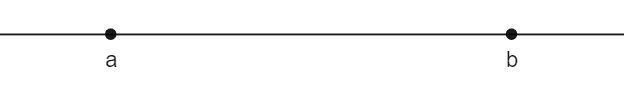
\includegraphics[scale=0.75]{interval}
  \end{figure}

  We call this set of subintervals $P$, and the ``length'' of the longest subinterval in $P$ is called the \textit{norm} or \textit{mesh} of $P$, $\max\{\abs{x_i-x_{i-1}} : 1\leq i \leq n\}$ denoted as $\abs{P}$. 
\end{frame}

\begin{frame}
  Then consider $$\sum_{i=1}^n f(t_i)(x_i-x_{x-1}), ~ t_i\in\sbr{x_{i-1},x_i}.$$ This summation can be interpreted graphically as the sum of rectangular areas, where $f(t_i)$ is the height and $(x_i-x_{i-1})$ is the length.

  \begin{figure}[h]
    \centering
    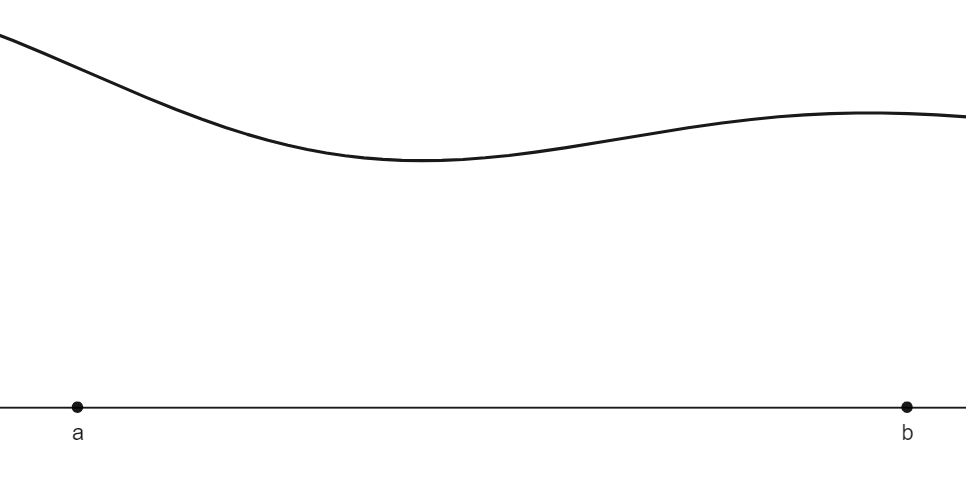
\includegraphics[scale=0.4]{firstsum}
  \end{figure}

\end{frame}

\begin{frame}
  Then consider what happens when we let $n$ become arbitrarily large. The partition of the interval $\sbr{a,b}$ would then be made of arbitrarily small subintervals, meaning their lengths approach zero. 
  
  Since $\abs{P}$ is the length of the longest subinterval, it too will approach zero. 

  So we say that as $n$ tends to infinity, or that $\abs{P}$ tends to zero, that the sum is equivalent to the definite integral of $f$ over $\sbr{a,b}$. So $$\lim_{\substack{ n\to \infty \\ (\abs{P}\to 0)}} \sum_{i=1}^n f(t_i)(x_i-x_{i-1}) = \int_a^b f(x)\dd{x}.$$

  \begin{figure}[h]
    \centering
    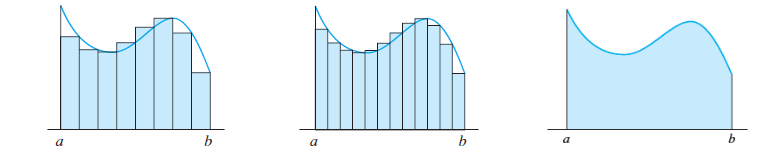
\includegraphics[scale=0.5]{improve}
  \end{figure}

\end{frame}

\section{Statement of the theorem}

\begin{frame}
  \frametitle{The statement}
  \begin{theorem}[Fundamental Theorem of Calculus]
    If $f : \sbr{a,b} \to \mathbb{R}$ is Riemann integrable, then:
    
    (1) $F$ given by $$F(x) = \int_a^x f(t)\dd{t}$$ is continuous.
    
    (2) Furthermore, $$\dv{x}F(x) = f(x)$$  whenever $f$ is continuous at $x$.
  \end{theorem}
  
\end{frame}
  
\begin{frame}
  \begin{theorem}[Antiderivative theorem]
    Again, let $f:\sbr{a,b}\to \mathbb{R}$ be Riemann integrable.

    (3) Let $G$ be any antiderivative of $f$, that is, $\dv{G}{x} = f(x)$. Then $$\int_a^b f(x)\dd{x} = G(b)-G(a).$$
  \end{theorem}

  So (1) states that the integral as a function is always continuous. I will not prove this, but I will give an intuitive explanation. Then (2) states that we can differentiate $F$ wherever $f$ is continuous, and (3) is our familiar result where we use an antiderivative to evaluate definite integrals.
\end{frame}

\section{The proof}

\begin{frame}
  \frametitle{The continuity of $F(x)$, intuitively}
  Here we will discuss how part (1) of the theorem works.
  
  Visually, the quantity $F(x)$ represents the \textit{accumulation} of the signed area under the graph of $f$ from $a$ to $x$. $$F(x) = \int_a^x f(t)\dd{t}$$

  \begin{figure}[h]
    \centering
    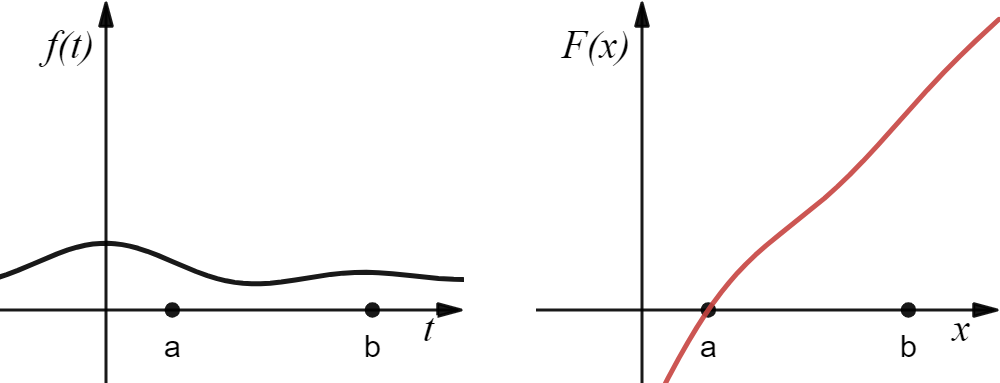
\includegraphics[scale=0.33]{accumulation}
  \end{figure}

\end{frame}

\begin{frame}
  Piecewise continuous example:

  \begin{figure}[h]
    \centering
    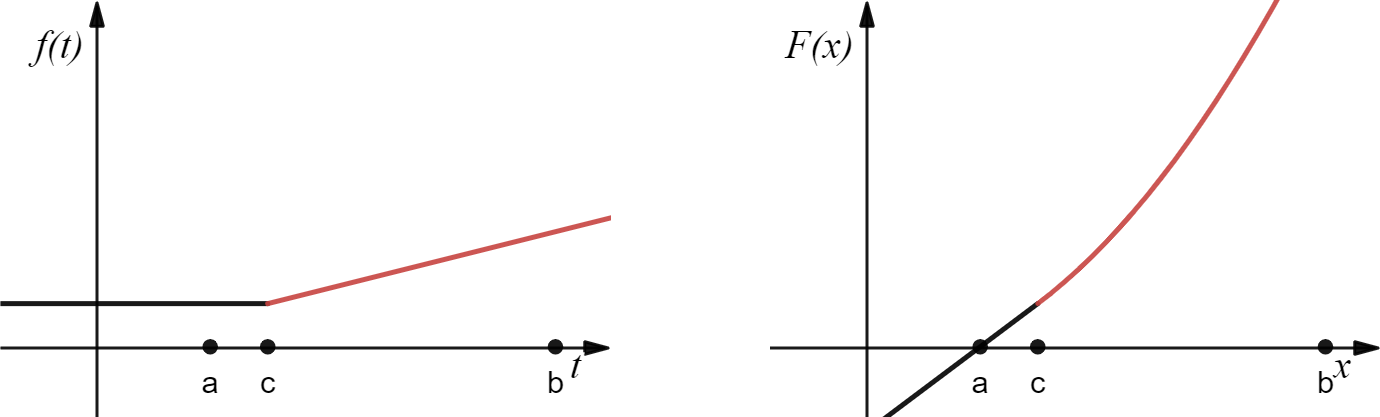
\includegraphics[scale=0.3]{piecewise}
  \end{figure}

  (Remember that $F(x) = \int_a^x f(t)\dd{t}$.)

\end{frame}

\begin{frame}

  We can imagine how $F$ is continuous whenever $f$ is, but how can we think about what happens when $f$ is discontinuous? An example:

  \begin{figure}[h]
    \centering
    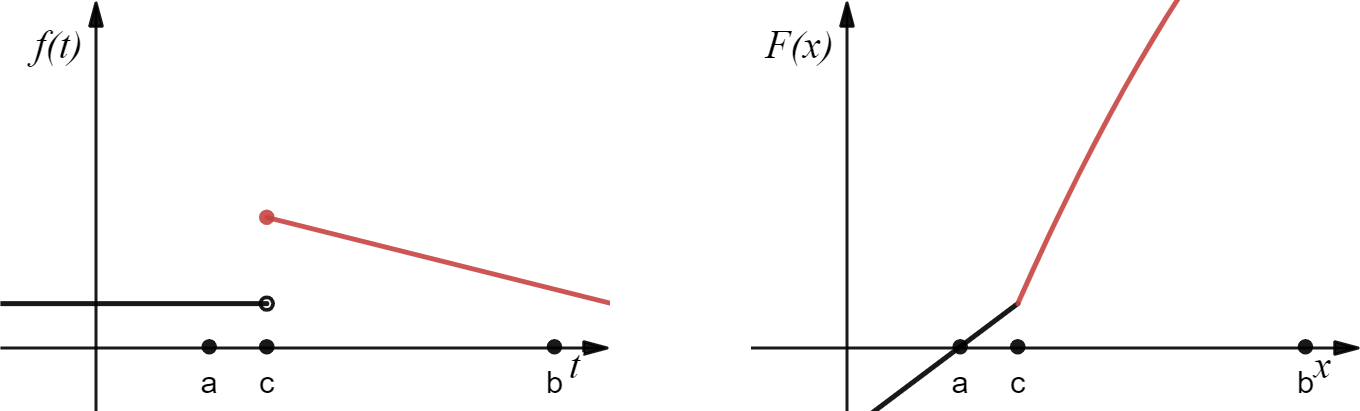
\includegraphics[scale=0.33]{discontinuous}
  \end{figure}

  Thus concludes our discussion of part (1) of the theorem, which states that $F$ is continuous.

\end{frame}

\begin{frame}
  \frametitle{Differentiating $F$ whenever $f$ is continuous}
  Now we move into part (2) of the theorem.

  By definition, $$\dv{F}{x} = \lim_{h\to 0}\frac{F(x+h)-F(x)}{h} = \lim_{h\to 0}\frac{\int_a^{x+h}f(t)\dd{t} - \int_a^x f(t)\dd{t}}{h}$$
  $$= \lim_{h\to 0} \frac{1}{h}\int_x^{x+h} f(t)\dd{t}.$$ We must show that this limit exists and is equal to $f(x)$.
\end{frame}

\begin{frame}
  Consider the following quantities \begin{align} m(x,h) &= \inf\{f(s) : \abs{s-x}\leq \abs{h}\} \\ M(x,h) &= \sup\{f(s) : \abs{s-x}\leq \abs{h}\}, \end{align} which can be graphically thought of as values that bound* $f$ in the neighborhood $\sbr{x-h,x+h}$.

  \begin{figure}[h]
    \centering
    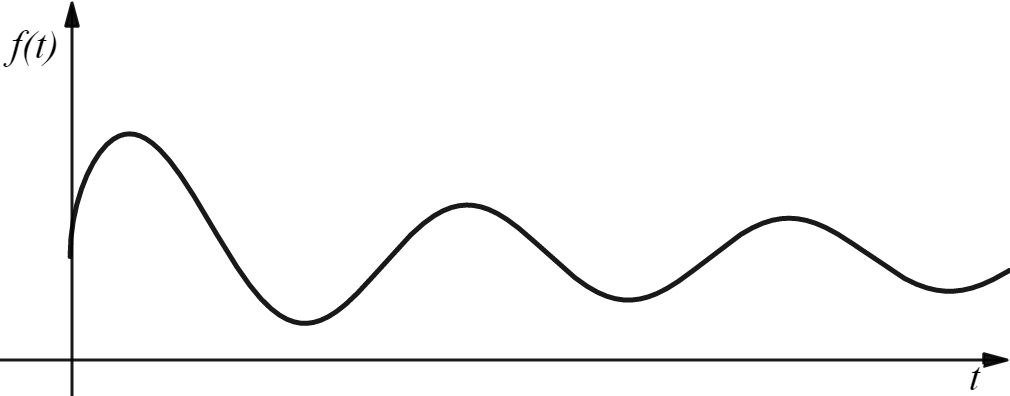
\includegraphics[scale=0.33]{neighborhood}
  \end{figure}
\end{frame}

\begin{frame}
  When $f$ is continuous at $x$, $m(x,h)$ and $M(x,h)$ converge to $f(x)$ as $h$ tends to $0$. We can imagine this working out with a convenient example.

  \begin{figure}[h]
    \centering
    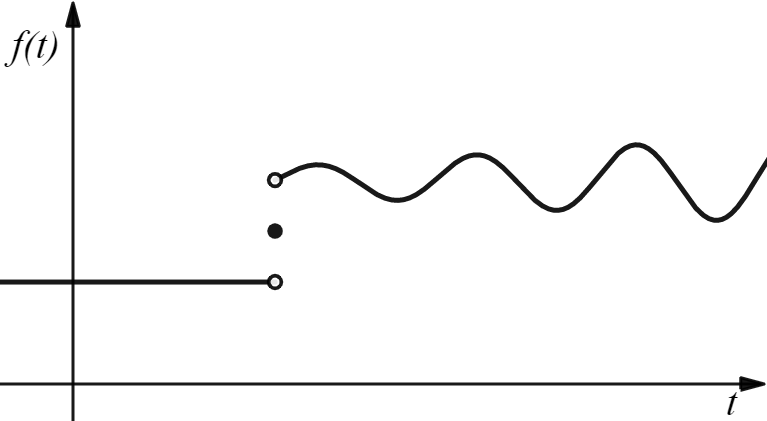
\includegraphics[scale=0.4]{wiggly}
  \end{figure}

  So more explicitly, $\displaystyle{\lim_{h\to 0} m(x,h) = f(x)}$ and $\displaystyle{\lim_{h\to 0} M(x,h) = f(x)}$.

\end{frame}

\begin{frame}
  We have that $$\int_x^{x+h} m(x,h) \dd{t} \leq \int_x^{x+h} f(t)\dd{t} \leq \int_x^{x+h} M(x,h)\dd{t}$$ since $m(x,h)\leq f(x)\leq M(x,h)$. 

  \begin{figure}[h]
    \centering
    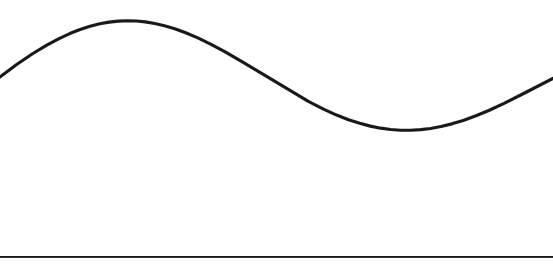
\includegraphics[scale=0.66]{squish}
  \end{figure}

\end{frame}

\begin{frame}
  Thus $$\frac{1}{h}\int_x^{x+h} m(x,h) \dd{t} \leq \frac{1}{h}\int_x^{x+h} f(t)\dd{t} \leq \frac{1}{h}\int_x^{x+h} M(x,h)\dd{t},$$ and notice that since $m(x,h)$ is constant with respect to $t$, we have that $$\frac{1}{h}\int_x^{x+h} m(x,h) = \frac{m(x,h)}{h}\br{x+h-x} = m(x,h).$$ Similarly $\frac{1}{h}\int_x^{x+h}M(x,h)\dd{t} = M(x,h)$.
\end{frame}

\begin{frame}
  So then $$m(x,h)\leq \frac{1}{h}\int_x^{x+h}f(t)\dd{t}\leq M(x,h),$$ and \textit{when $f$ is continuous at $x$} we can use the fact that $m(x,h)$ and $M(x,h)$ converge to $f(x)$ as $h$ tends to zero to find that $$\lim_{h\to 0}m(x,h)\leq \lim_{h\to 0} \frac{1}{h}\int_x^{x+h}f(t)\dd{t} \leq \lim_{h\to 0}M(x,h)$$ becomes $$f(x) \leq \dv{F}{x} \leq f(x) \iff \dv{x}F = f(x) ,$$ which is part (2) of the theorem.
\end{frame}

\begin{frame}
  \frametitle{Using antiderivatives to compute definite integrals}
  We are (finally) beginning discussion of part (3) of the theorem. This part is going to be a little more algebraic.

  We need to define what an antiderivative is. An antiderivative $G$ of $f : \sbr{a,b}\to \mathbb{R}$ satisfies $$G^{\prime}(x) = f(x)$$ for all $x\in\sbr{a,b}$. 

  A nice thing to think about is \textit{when} functions have antiderivatives.
\end{frame}

\begin{frame}
  We also have that antiderivatives $G(x)$ differ from the indefinite integral $\int_a^x f(t)\dd{t}$ by a constant, that is, $$G(x) = \int_a^x f(t)\dd{t} + C$$ for some constant $C$.

  Similarly as before, partition $\sbr{a,x}$, which is only part of $\sbr{a,b}$, into $n$ subintervals, where $a = x_0 < x_1 < \cdots < x_{n-1} < x_n = x$.
\end{frame}

\begin{frame}
  Consider the following quantity $$\frac{G(x_k)-G(x_{k-1})}{x_k-x_{k-1}},$$ and note that due to the mean value theorem, the above quantity is equal to $G^{\prime}(t_k) = f(t_k)$, where $t_k\in\sbr{x_{k-1},x_k}$. This is true \textit{no matter how small the subinterval $\sbr{x_{k-1},x_k}$ is}.
  
  So then we have $$G(x_k)-G(x_{k-1}) = f(t_k)(x_k-x_{k-1})$$
\end{frame}

\begin{frame}
  Then we can sum over all of the subintervals, so $$\sum_{k=1}^n f(t_k)(x_k-x_{k-1}) = \sum_{k=1}^n G(x_k)-G(x_{k-1})$$ \begin{multline*}= \br{G(x_1)-G(x_0)} + \br{G(x_2)-G(x_1)} + \br{G(x_3)-G(x_2)} \\ + \cdots + \br{G(x_{n-1})-G(x_{n-2})} + \br{G(x_n)-G(x_{n-1})}\end{multline*}
  $$ = G(x_n)-G(x_0) = G(x) - G(a)$$
\end{frame}

\begin{frame}
  Since $G(x_k)-G(x_{k-1}) = f(t_k)(x_k-x_{k-1})$ holds regardless of the size of the subinterval $\sbr{x_{k-1},x_k}$, we can consider taking the following limit: $$\lim_{n\to \infty}\sum_{k=1}^n f(t_k)(x_k-x_{k-1}) = \lim_{n\to \infty}  G(x) - G(a)$$

  But the left hand side is the definition of the integral from $a$ to $x$ of $f(t)$, and the right hand side remains unchanged. So then the previous equation becomes $$\int_a^x f(t)\dd{t} = G(x)-G(a).$$
\end{frame}

\begin{frame}
  So $$G(x) = \int_a^x f(t)\dd{t} + G(a),$$ where $G(a)$ is a constant. This proves part (3) of the theorem. 

  Notice that if we go back one step and evaluate both sides of the equation at $x=b$, we get the familiar formula we learned to evaluate integrals. $$\int_a^b f(t)\dd{t} = G(b)-G(a)$$
\end{frame}

\section{Closing remarks and/or questions}

\begin{frame}
  \frametitle{Extra slide in case I wanted to write something down}
\end{frame}

\end{document}